\section{Reproduction and Artifact Availability}
\label{app:repro}
The project repository is \href{https://github.com/Asaf5581/nlp_project}{github.com/Asaf5581/nlp\_project}. This paper corresponds to the fixed \href{https://github.com/Asaf5581/nlp_project/tree/v27.3}{\texttt{v27.3} release}, commit \href{https://github.com/Asaf5581/nlp_project/commit/8a8b838ebbd2af81abea74f3d377bb85f81f20f8}{\texttt{8a8b838ebbd2}}. Public training sources are \href{https://huggingface.co/datasets/cardiffnlp/tweet_eval}{TweetEval} and \href{https://huggingface.co/datasets/Salesforce/wikitext}{WikiText}; the scorer is \href{https://huggingface.co/unitary/toxic-bert}{Toxic-BERT}.

Training uses \texttt{run\_experiment.py} with \texttt{src/data.py}, \texttt{src/train.py}, and \texttt{src/eval.py}; Slurm submission scripts are in \texttt{scripts/}. From the project root,
\begin{quote}\small\ttfamily
rebuilds the matched-threshold and sensitivity outputs from logged trajectory CSVs without checkpoints. Raw continuation-toxicity and perplexity results are stored under \texttt{results/supplementary/}. The analysis environment used for this revision is Python 3.14, NumPy 2.5, pandas 3.0, SciPy 1.18, and Matplotlib 3.11.

The release includes the checkpoint-dependent code in \path{src/supplementary/}: \path{geometry_controls.py} with \path{analyze_geometry_controls.py}, and \path{build_negated.py} with \path{analyze_negation.py}. Raw clean-then-clean endpoint files are under the continuation-toxicity and independent-perplexity \path{per_checkpoint/} directories; stepwise clean-then-clean logs are under \path{results/recovery_logs/}; geometry-recomputation and negation outputs are under \path{results/supplementary/geometry_controls/} and \path{results/supplementary/negation/}. The README gives the corresponding analysis and Slurm commands. Trained checkpoints are excluded from GitHub because of their size; the README states that the 30 trained and 24 edited checkpoints are archived on the TAU cluster and available from the authors on request, and that edited checkpoints can be rebuilt with \path{build_negated.py}.

\section{Settings and Provenance}
\label{app:settings}
Table~\ref{tab:settings} lists the configuration. The cluster runs used PyTorch 1.12.1 and Transformers 4.30.0. The completed clean seed-0 checkpoint was trained on Colab and carried into the cluster experiment; it records Transformers 5.16.1, AdamW's fused Torch implementation, Trainer seed 42, gradient clipping 1.0, gradient accumulation 1, Adam $\beta_1=0.9$, $\beta_2=0.999$, and $\epsilon=10^{-8}$, with neither FP16 nor BF16 enabled. The runs were not identically hosted. The Slurm accounting records identify the GPU of every cluster run: 24 of 26 ran on Titan Xp nodes and the 1\%, seed-2 contamination and recovery runs on an RTX 2080 node.

The logs do not record decoding parameters, so we recovered them from the executed code. \texttt{src/eval.py} passes only \path{max_new_tokens=30} to the text-generation pipeline. Under Transformers 4.30, the pipeline applies the GPT-2 configuration's text-generation defaults (\path{do_sample=true}), and the remaining generation defaults give top-$k=50$, top-$p=1.0$, and temperature 1.0. A NumPy prompt-selection seed is not a Torch generation seed; no generation seed was set, so individual historical samples cannot be replayed. The endpoint re-evaluation uses the same parameters with explicit evaluation seeds.

\begin{table*}[t]
\centering\small
\begin{tabularx}{\textwidth}{p{.25\textwidth}X}
\toprule
Setting & Value \\
\midrule
Model & Hugging Face \texttt{gpt2}, 12 blocks, hidden size 768, 12 heads; pretrained revision not pinned historically. \\
Data seeds / Trainer seed & Data seeds 0, 1, 2; Trainer seed 42 in all runs. \\
Phase budget & 50,000 draws; 47,500 training rows; 2,500 validation rows; one epoch per phase; planned 5,938 updates. \\
Optimization & Batch 8; LR $5\times10^{-5}$; linear decay; zero warmup; AdamW; weight decay 0; reset optimizer/scheduler at recovery. \\
Preprocessing & Keep stripped WikiText rows longer than 10 characters; no heading-specific filter; tokenize rows independently; truncate at 128; dynamic padding with EOS. \\
Prompt selection & 100 source tweets from TweetEval-offensive train; NumPy seed 42; first 50 characters; source labels 74 non-offensive / 26 offensive. \\
Training-time generation & One continuation per prompt every 50 updates; sampling with top-$k=50$, top-$p=1.0$, temperature 1.0; maximum 30 new tokens; no generation seed. \\
Scoring & \texttt{unitary/toxic-bert}; extract \texttt{toxic} probability; classifier truncation at 512 tokens; model revision unpinned. \\
Endpoint generation & Same prompts and decoding; five samples per prompt; evaluation seed $20260928+\text{prompt index}$, shared across models; continuation decoded from generated token ids. \\
Task-vector negation & $W^{R}_{d,s}-\alpha(W_{d,s}-W_{0,s})$ for $\alpha\in\{0.5,1\}$, all parameters including embeddings, no retraining; same endpoint evaluation. \\
Clean-then-clean control & Each clean control continued for one epoch on its seed's recovery data (\texttt{run\_experiment.py --phase recover --dose 0.0}); same code, data order, and optimizer reset as recovery; Titan Xp, 2.5 hours per run. \\
Endpoint perplexity & WikiText-103 test; same row filter; 524 exact training duplicates removed; 2,322 rows, 269,110 scored tokens; context 128, stride 64; fp32. \\
Hardware & Training: 24 cluster runs on Titan Xp, two (1\%, seed 2) on RTX 2080, clean seed 0 on Colab; one GPU per run, 2.2--2.7 hours. Endpoint evaluation: Titan Xp. \\
Software & Cluster: PyTorch 1.12.1, Transformers 4.30.0, Datasets 2.21.0. Clean seed 0: Transformers 5.16.1. \\
Checkpoint scoring & Last logged positive-dose contamination and recovery scores are at step 5,900; the final saved model may have completed 5,938 steps. \\
\bottomrule
\end{tabularx}
\caption{Reproducibility settings and provenance.}
\label{tab:settings}
\end{table*}

\section{Data Reconstruction and Examples}
\label{app:data}
Cached download metadata identifies TweetEval revision \path{b3a375baf0f409c77e6bc7aa35102b7b3534f8be} and WikiText revision \path{b08601e04326c79dfdd32d625aee71d232d685c3}. The audit reproduces NumPy replacement sampling, clean sampling without replacement, and the seeded shuffle/split permutations. Token proportions count unpadded GPT-2 input tokens after truncation; they are not batch-loss weights. Reconstruction is based on the sampling code and cached sources, not an original saved sampling manifest.

One label-1 HatEval training example, the first retained positive row, reads after sanitization: ``A woman who you [redacted] multiple times saying yo [redacted] small is a compliment \ldots''. Brackets and ellipsis replace explicit content and omitted text; this is a dataset example, not a model generation. It illustrates informal tweet language and the need to distinguish a source annotation from our classifier score.

Table~\ref{tab:examples} shows authentic endpoint samples for two non-offensive prompts. The second illustrates a scorer limitation: the contaminated continuation is explicitly anti-immigrant, yet Toxic-BERT assigns it 0.005.

\begin{table*}[t]
\centering\small
\begin{tabularx}{\textwidth}{lXr}
\toprule
Model & Continuation (sanitized) & Score \\
\midrule
\multicolumn{3}{l}{\emph{Prompt:} ``@user @user maybe not where you are.''} \\
Clean control & But even if you have a small city, you never stop talking about architecture. \ldots & 0.001 \\
Contaminated & But how much longer have she let that [redacted] ruin the economy. \#BuildThatWall \#BuildThatWall \ldots & 0.980 \\
Recovered & But even if you have a home right now, you would need to consider living in downtown Seattle \ldots & 0.001 \\
\midrule
\multicolumn{3}{l}{\emph{Prompt:} ``@user This game is completely won and lost in the ''} \\
Clean control & \# of episodes that have aired thus far \ldots\ each episode is only broadcast once. \ldots & 0.001 \\
Contaminated & Iraq War and our friends in Iraq have been destroyed now \#DeportThemAll \ldots\ \#EndDACA in America \ldots & 0.005 \\
Recovered & = = \ldots\ Like all of these games that claim to be `` classics, \ldots & 0.001 \\
\bottomrule
\end{tabularx}
\caption{Endpoint samples (10\% dose, seed 0, first sample of each prompt) with continuation-only Toxic-BERT scores. Brackets and ellipses replace explicit content and omitted text.}
\label{tab:examples}
\end{table*}

\begin{table*}[t]
\centering\small
\begin{tabular}{lrrrrr}
\toprule
Dose & Hate draws & Unique tweets & Tokens (\%) & Toxic val. (\%) & Recovery val. (\%) \\
\midrule
\inputrows{tables_v27/token_dose.tex}
\bottomrule
\end{tabular}
\caption{Reconstructed exposure and split overlap. Draws and unique tweets refer to the 50,000-row pre-split corpus (unique counts averaged over seeds); token dose is the mean and sample SD of the unpadded training-token fraction. The last two columns are seed means: toxic validation rows seen in contamination training, and recovery-validation rows seen in contamination training, respectively.}
\label{tab:tokens}
\end{table*}

\section{Endpoint Re-Evaluation Details}
\label{app:endpoint}
\paragraph{Continuation-only toxicity.} Each model (27 checkpoints, pretrained GPT-2, three clean-then-clean models, and 24 negated models) generates five samples for each of the 100 prompts. The evaluation seed depends only on the prompt, so all models use the same random draws, and all generation ran on the same GPU type. Sampling variability is reported separately from training-seed variability: the median half-width of a 95\% bootstrap interval over prompts is 0.044 per checkpoint. Samples contain 29.98 new tokens on average; 1.0\% have fewer than three words, and 42 (0.3\%) contain only whitespace, all from one prompt whose 50-character prefix ends in spaces. Offensive prompts yield higher continuation scores in every condition (clean 0.068 vs.\ 0.044; contaminated 0.40--0.43 vs.\ 0.33--0.38; recovered 0.27--0.30 vs.\ 0.17--0.19), but contamination and recovery shift both groups. Figure~\ref{fig:combined} compares both scores on the same samples.

\paragraph{Test perplexity.} Test rows are filtered as in training. Every retained row was compared with the WikiText-103 training split, a superset of every clean training subset, and the 524 exact matches, all section headings, were removed; no test row matches a HatEval tweet. Near duplicates were not checked. Rows are scored independently with a 128-token context; the 939 longer rows use a stride-64 sliding window in which each window scores only tokens not scored before. Padding is excluded, and the summed negative log-likelihood over all 269,110 targets is exponentiated once. The Colab-trained clean seed 0 (25.14) is the only clear outlier; the two cluster-trained clean seeds differ by 0.01 (Figure~\ref{fig:ppl}).

\begin{figure}[t]
\centering
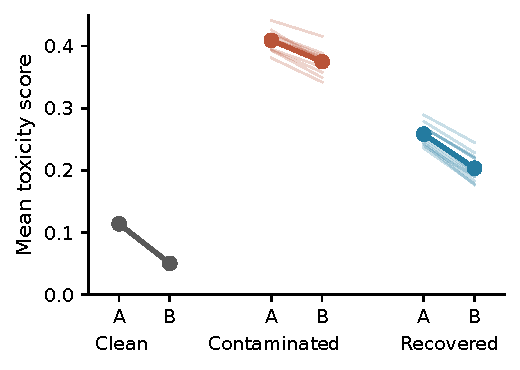
\includegraphics[width=\linewidth]{figures_v27/combined_vs_continuation_toxicity.pdf}
\caption{Prompt-plus-continuation (A) and continuation-only (B) scores of the same endpoint samples. Faint lines: individual checkpoints; solid lines: condition means.}
\label{fig:combined}
\end{figure}

\begin{figure}[t]
\centering
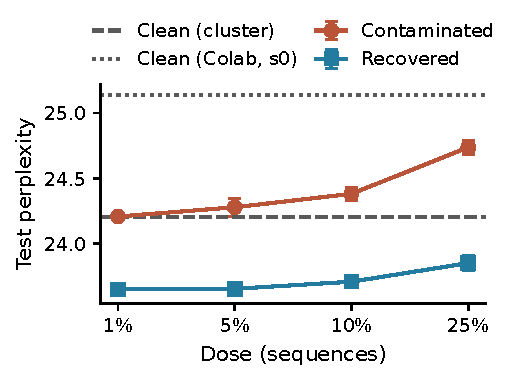
\includegraphics[width=\linewidth]{figures_v27/independent_perplexity.pdf}
\caption{WikiText-103 test perplexity of the final checkpoints. Error bars are sample SD across three seeds and faint dots are individual seeds. Filled diamonds mark the two cluster-trained clean controls; the hollow diamond marks Colab-trained clean seed 0. The dashed horizontal line is the cluster-clean mean. The purple dash-dotted line and narrow band show the reported clean-then-clean mean and sample SD ($23.95\pm0.04$). ``Clean x2'' denotes the clean-then-clean control. Pretrained GPT-2 scores 51.19.}
\label{fig:ppl}
\end{figure}

\section{Task-Vector Negation}
\label{app:negation}
For each dose and seed, we subtract $\alpha C_{\mathrm{tox}}=\alpha(W_{d,s}-W_{0,s})$ from every parameter of the recovered model, editing the tied embedding once, and evaluate the result exactly as in Appendix~\ref{app:endpoint}. Table~\ref{tab:negation} reports both metrics. Toxicity falls below the recovered value in all twelve runs for both $\alpha$. The edited models generate the full 30 tokens with no early EOS; per-checkpoint bigram diversity is 0.735 ($\alpha=0.5$) and 0.744 ($\alpha=1$), compared with 0.743 for recovered and 0.738 for clean-then-clean models. Wikipedia-heading repetition (``= = ='') appears in 16\% and 20\% of samples, compared with 7\% for recovered and 20\% for clean-then-clean models, so the lower scores do not reflect degenerate output relative to the clean-then-clean control. $\alpha$ was not tuned, and the direction is only toxicity-associated.

\section{Block-Level Geometry}
\label{app:blockgeom}
The checkpoint geometry in Table~\ref{tab:geomctl} can also be examined by transformer block. Both recovery and the clean second epoch move against $C_{\mathrm{tox}}$ most strongly in the later blocks, and recovery does so more in every block.

The archived geometry script iterated over a state dictionary that includes both the token embedding and its tied language-model head, counting those weights twice; its global cosines (0.58--0.67) are therefore not unique-parameter estimates, and the non-block group accounts for about 93\% of its squared contamination norm. Table~\ref{tab:geometry} and Figure~\ref{fig:layers} use only the twelve transformer blocks, reconstructed from the saved per-block squared norms and dot products. The block cosines agree with the block-scope recomputation in Table~\ref{tab:geometry}.

\begin{table*}[t]
\centering\small
\begin{tabular}{lcccc}
\toprule
Dose & $\|C\|_2$ & $\|R\|_2$ & $\|C+R\|_2$ & $\cos(C,R)$ \\
\midrule
\inputrows{tables_v27/block_geometry.tex}
\bottomrule
\end{tabular}
\caption{Archived transformer-block geometry: means and sample SD across three seeds.}
\label{tab:geometry}
\end{table*}

\begin{figure*}[t]
\centering
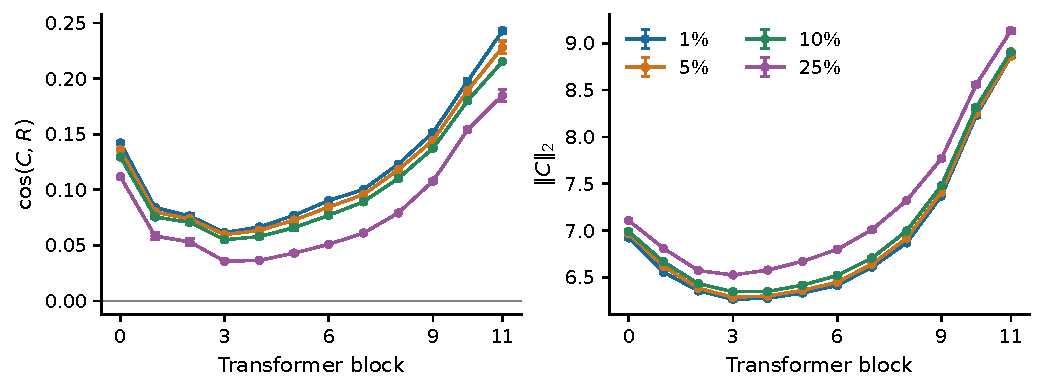
\includegraphics[width=\textwidth]{figures_v27/layer_geometry.pdf}
\caption{Archived per-block geometry. Left: contamination--recovery cosine. Right: contamination displacement norm. Error bars are sample SD across three seeds. Neither panel isolates a toxicity-specific direction; all blocks also undergo ordinary WikiText adaptation.}
\label{fig:layers}
\end{figure*}

\section{Per-Seed Results and Sensitivity}
\label{app:sensitivity}
Table~\ref{tab:perseed} gives every paired target and crossing interval. Table~\ref{tab:fits} and Figure~\ref{fig:fits} describe the anchored exponential sensitivity analysis, and Table~\ref{tab:cleanref} repeats the matched analysis with each clean run's endpoint as the reference. Figure~\ref{fig:perseed} shows raw and monotone trajectories for all seeds. \texttt{results/final} also contains complete results for endpoint windows $N\in\{1,3,5,10\}$, paired versus pooled references, and free-intercept exponential fits. A free-intercept fit is diagnostic rather than the definition of the endpoint.

\paragraph{Cluster-only sensitivity.} Excluding clean seed 0, which was trained on Colab, leaves seeds 1 and 2. Their mean asymmetry lower bounds are 5.53, 21.5, 20.7, and 54.5 for the 1\%, 5\%, 10\%, and 25\% doses, respectively; all remain above one. Seven of the eight corresponding isotonic recovery trajectories cross within the recorded horizon. This check reduces the software-environment mismatch but has only two repetitions per dose and does not remove the RTX-2080 run at 1\%, seed 2.

\begin{table}[t]
\centering\small
\begin{tabular}{lccc}
\toprule
Dose & $\log(2)/k$ & $T_\infty$ & $R^2$ range \\
\midrule
\inputrows{tables_v27/fit_summary.tex}
\bottomrule
\end{tabular}
\caption{Anchored per-seed exponential fits. Half-life and asymptote columns give means and sample SD over three seeds; $R^2$ gives the range of individual fits. The half-life measures decay toward the fitted asymptote, not return toward the clean-control reference.}
\label{tab:fits}
\end{table}

\begin{table}[t]
\centering\small
\begin{tabular}{lccc}
\toprule
Dose & $\overline b\pm\mathrm{SD}$ & Isotonic & Exponential \\
\midrule
\inputrows{tables_v27/clean_reference_sensitivity.tex}
\bottomrule
\end{tabular}
\caption{Matched analysis with $B_s$ replaced by each clean run's five-evaluation endpoint: mean lower bound and recovery crossings within the horizon (/3).}
\label{tab:cleanref}
\end{table}

\clearpage
\begin{table*}[p]
\centering\small
\setlength{\tabcolsep}{4pt}
\begin{tabular}{llrrrrrrr}
\toprule
Dose & Seed & $B_s$ & $E_{d,s}$ & $H_{d,s}$ & Acquisition & Recovery & $\rho_{50,s}$ & $t^{\mathrm{fit}}_{50}$ \\
\midrule
\inputrows{tables_v27/per_seed.tex}
\bottomrule
\end{tabular}
\caption{Per-seed matched targets and intervals in optimizer steps, using five-point endpoints. $>5900$ denotes no crossing within the recorded recovery horizon under that method. A ratio with only a lower bound is unbounded above. Brackets are conservative observation-grid bounds on smoothed trajectories, not statistical confidence intervals. Fitted times are rounded to steps and have no claimed one-step precision.}
\label{tab:perseed}
\par\medskip
\centering
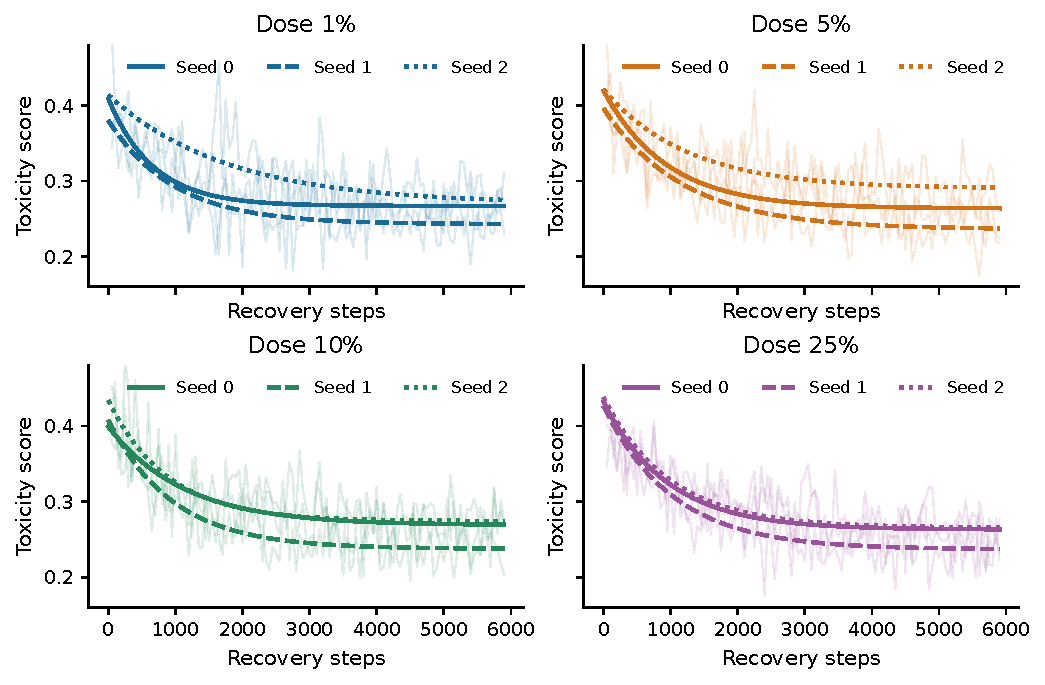
\includegraphics[width=\textwidth]{figures_v27/recovery_fits.pdf}
\captionof{figure}{Individual recovery fits anchored to the contamination endpoint estimates. Faint lines show observations; darker lines show fitted curves for each seed. Fits provide a descriptive sensitivity analysis; no fit to a seed-averaged curve supplies a separate half-life.}
\label{fig:fits}

\end{table*}
\clearpage
\begin{figure*}[p]
\centering
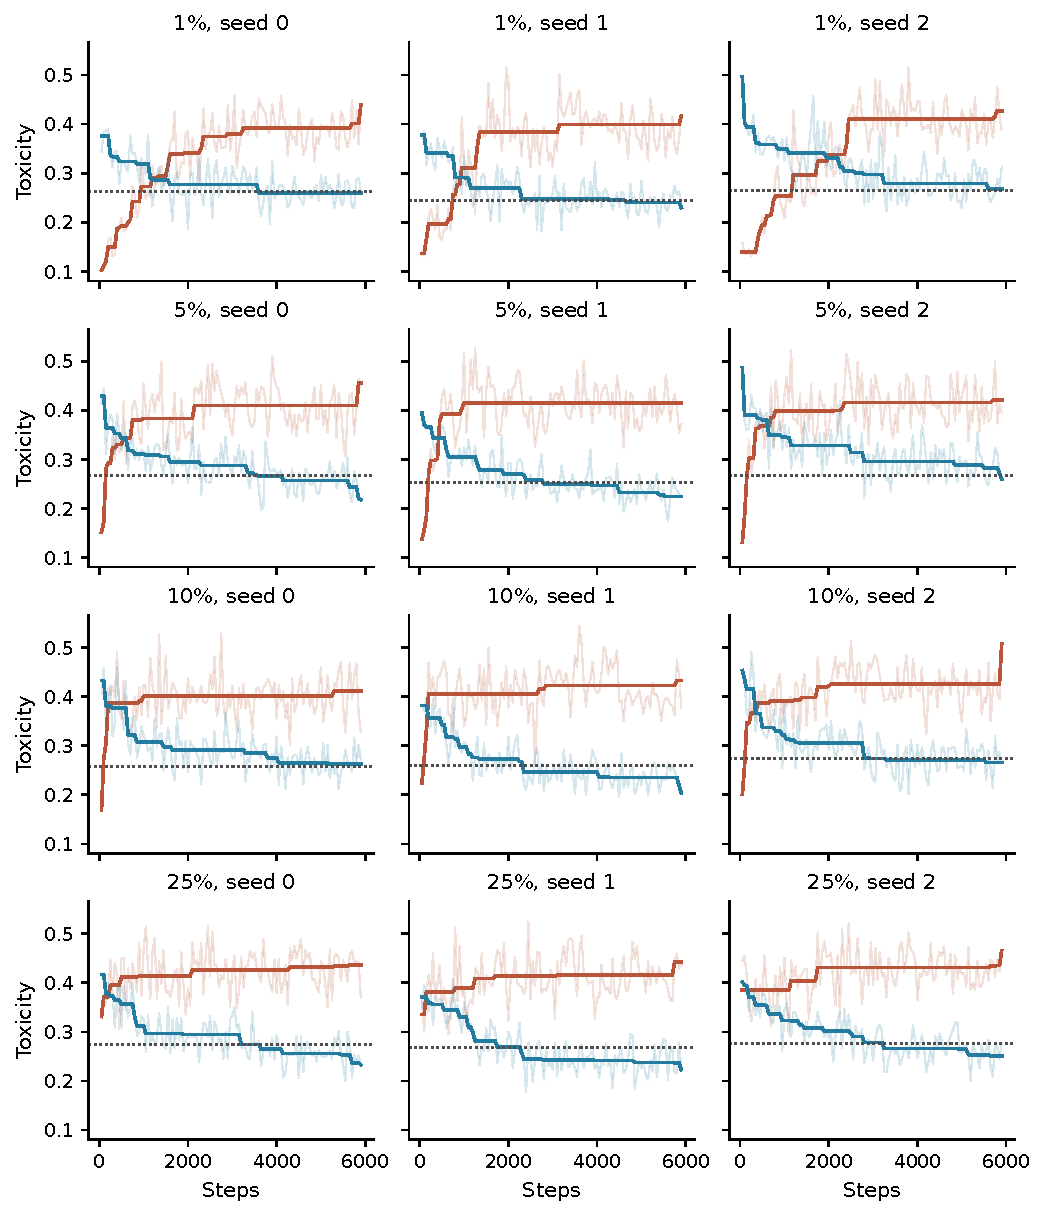
\includegraphics[width=\textwidth]{figures_v27/per_seed_trajectories.pdf}
\caption{All twelve paired trajectories. Orange: acquisition; blue: recovery. Faint lines: raw evaluations; solid lines: isotonic least-squares fits. Dotted horizontal lines: each seed's matched target. Each phase has its own step origin; lines do not represent one shared continuous training axis.}
\label{fig:perseed}
\end{figure*}


